\documentclass[10pt,print]{article}

\usepackage{amsmath}
\usepackage{amssymb}
\usepackage{authblk}
\usepackage[top=0.75in,left=0.75in,right=0.75in,bottom=1in]{geometry}
\usepackage{times}
\usepackage{graphicx}
\usepackage{subcaption}
\usepackage{hyperref}
\usepackage{cleveref}
\usepackage{xcolor}
\usepackage[numbers,sort&compress]{natbib}

\pagenumbering{gobble}

\newcommand{\ned}[1]{\textcolor{red}{#1}}
\newcommand{\utilde}[1]{\underset{\widetilde{}}{#1}}

\title{Hyper-Reduction Approaches for Contact Modeling with Small
  Tangential Displacements: Applications for a Bolted Joint}
\author[1]{Nidish Narayanaa Balaji\thanks{nb25@rice.edu}}
\author[2]{Tobias Dreher\thanks{tdreher.ahausen@web.de}}
\author[2]{Malte Krack\thanks{malte.krack@ila.uni-stuttgart.de}}
\author[1]{Matthew R. W. Brake\thanks{brake@rice.edu}}
\affil[1]{Department of Mechanical Engineering, William Marsh Rice
  University, Houston, TX 77005, USA}
\affil[2]{Institute of Aircraft Propulsion Systems, University of
  Stuttgart, Keplerstraße 7, 70174 Stuttgart, Germany}

\begin{document}
\maketitle{}

% \begin{abstract}
%   This paper considers the reduced order interface modeling of
%   mechanically contacting interfaces using distributions of surface
%   field quantities on the interface at different stages along
%   non-linear simulations. Focusing primarily on small (tangential)
%   displacement compliant contacts, two approaches are formulated and
%   compared for merits and limitations in applicability. The first is a
%   reformulation of the stiffness-preserving RBE3 constraint elements
%   (in ANSYS terminology) using a least-squares approximation of the
%   constraint equilibrium condition. Although RBE3 is extensively used
%   in the community, the least-squares condition makes the current
%   formulation more physically meaningful than conventional
%   implementations. The second approach uses interface remeshing for
%   developing a reduced order representation of the
%   interface. Reference states of the interface characterized as
%   surface fields of the relevant dynamic quantities (tractions and
%   dissipation fluxes) are used to formulate the reduced order model in
%   both approaches (the patches for the RBE3 elements and the reduced
%   order mesh for the remeshing). These reference states are evaluated
%   by conducting a limited number of preparatory nonlinear simulations
%   such as responses to static prestress and quasi-static load
%   cases. Retaining consistency with the virtual work done in the
%   interface, this approach offers reduction while at the same time
%   preserving the interpretation of the equations of motion. These are
%   termed hyper-reduction since the non-linear forces in both of the
%   above approaches are computed in the reduced domain directly. For
%   comparisons, the paper presents applications of the two approaches
%   for the reduced order modeling of a bolted lap joint benchmark.
% \end{abstract}

\textbf{Keywords:} Interface reduction, hyper-reduction, jointed
structures

\section{Introduction and Motivation}
\label{sec:intr-motiv}

Model order reduction of the non-linear dynamical models of
structures with frictional contacts is of high importance in making
simulations of such systems tractable. Even for relatively
simple bolted structures, the representational requirements as well as
the amount of non-linear evaluations necessary can make the system
very large and very expensive for simulations. Projection-based
techniques for model order reduction (see, for
instance~\cite{mitra2016adaptive}), which are based on finding an
appropriate reduced representation of the solution in a lower-rank
subspace (and solving the problem there), are a very popular
  approach in the literature. One of the main drawbacks with such
approaches is that it is generally not trivial to establish a reduced
representation of non-linearities on the chosen subspace itself. In
other words, evaluation of non-linearities in such models is conducted
by first transforming the unknowns into the full-order model,
evaluating the non-linearities, and then transforming them back into
the reduced domain. This procedure, while beneficial for a lot of
cases, becomes computationally cumbersome when it comes to very large
models wherein the evaluation of the non-linear function becomes an
important computational bottleneck. In order to alleviate this issue,
there have been several hyper-reduction approaches (see, for
  instance~\cite{ryckelynck_priori_2005}), which seek to develop
reduced order modeling strategies with the non-linearities completely
represented in the reduced domain itself. One promising approach for
this is to develop a data-based representation of the non-linearity on
the subspace (see~\cite{jain2019hyper} for an application) based on
several non-linear function evaluations on the full-order model. Such
an approach, however, suffers from input-level dependence, i.e., the
trained model performs only as good as the training data-set.

The current paper, following previous
efforts~\cite{dreher2020gerrymandering}, explores model reduction
through the development of reduced representations of the interface
while retaining the physical meaning of the degrees-of-freedom of the
reduced model. This allows for relatively easy definitions of the
non-linearities consistently in the reduced domain, thereby avoiding
the need to transform back to the full problem. Two approaches are
presented with their merits and shortcomings discussed: (1) an
improved whole-joint formulation (similar to the ones used
in~\cite{lacayo2019updating}) applied to regions on the interface
selected based on a binned field objective; and (2) an interface
remeshing approach based on efficient representation of a continuous
field objective.

\section{Description of Approaches}
\label{sec:descr-appr}

As already mentioned, the two approaches are closely tied together in
the sense that both are aimed at developing a representation of the
interface that best represents a particular field quantity over the
interface (contact pressure, dissipation fluxes, etc.). Therefore, a
scalar-valued field objective, denoted $\mathcal{P}(\utilde{x})$
  in the following, has to first be identified so that the reduced
  model can be developed.

\begin{figure}[!h]
  \centering
  % \boxed{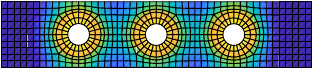
\includegraphics[width=0.49\linewidth]{FIGS/REF}}
  \boxed{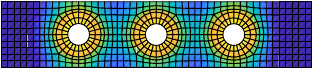
\includegraphics[width=0.49\linewidth]{8621_bal_Fig1}}  
  \caption{Reference mesh. The static contact pressure mapped to [0,
    1], used as the field objective in the following, is denoted using
    colours.}
  \label{fig:iraref}
\end{figure}

All of the results shown in the following are based on the
  interfacial mesh shown in~\cref{fig:iraref}, which corresponds to
  the bolted joint interface for a finite-element model of the
  Brake-Reu{\ss} Beam (BRB), a three-bolted lap-joint
  structure~\cite{brake2017mechanics}. The field objective that will
  be used here will be the normal contact pressure from static
  bolt-prestress simulations (with each bolt applying a prestress of
  11.58 kN) used as the field objective (re-ranged to [0,1] and
  denoted using color here).

\subsection{Whole Jointed Approach Based on Binned Field Objective}
\label{sec:whole-joint-appr}

\begin{figure}[!h]
  \centering
  \begin{subfigure}{0.5\linewidth}
    \centering
    % \boxed{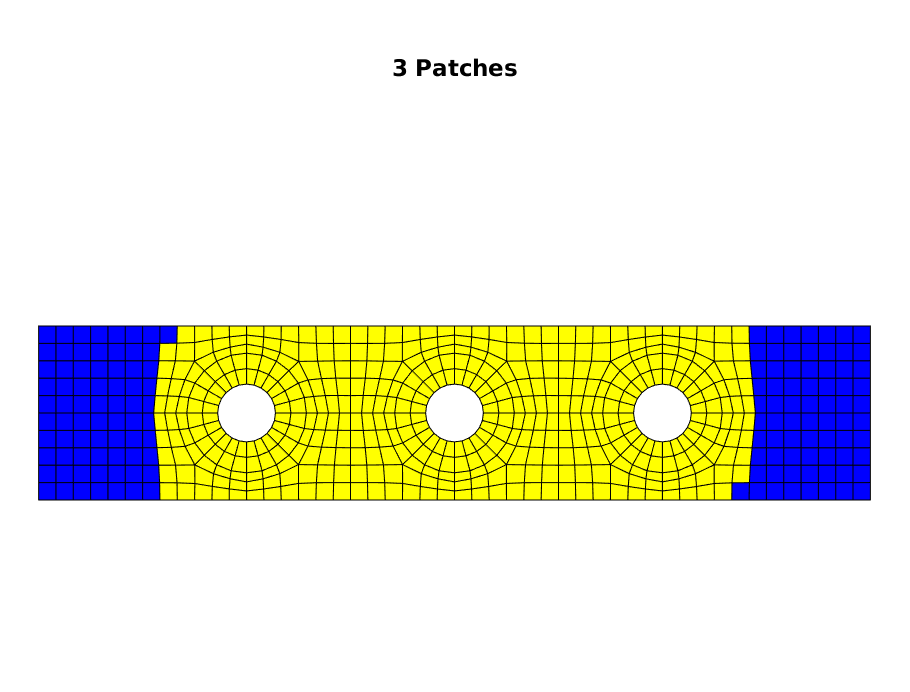
\includegraphics[width=0.9\linewidth,trim={1cm 2.95cm 1cm
    %     5.2cm},clip]{{{FIGS/P11580_S-6.00_2LEV_3PATCH_MESH}}}}
    \boxed{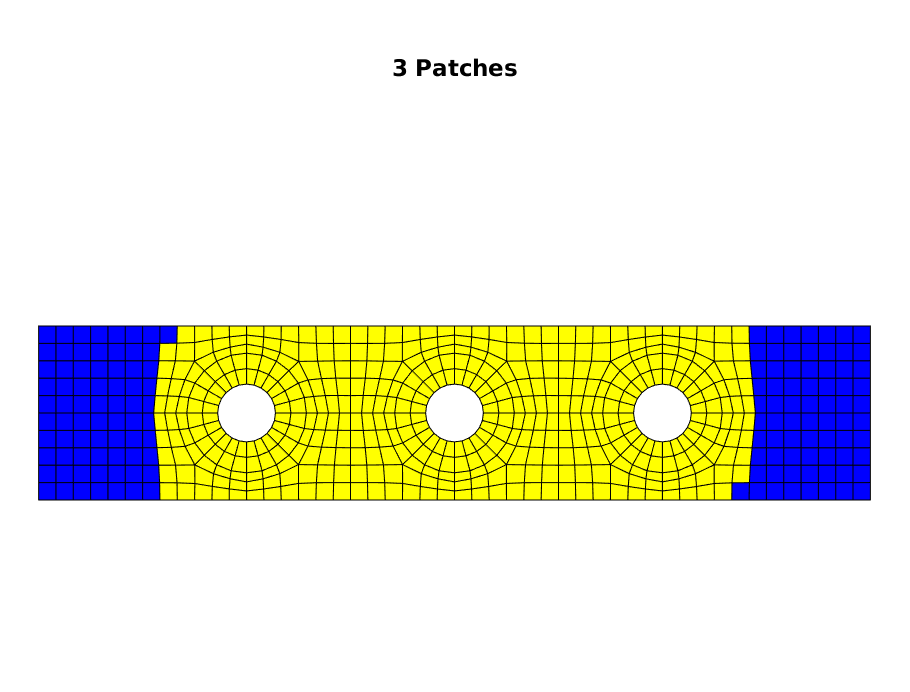
\includegraphics[width=0.9\linewidth,trim={1cm 2.95cm 1cm
        5.2cm},clip]{8621_bal_Fig2a}}
    \caption{2 Levels (3 Patches)}
  \end{subfigure}%
  \begin{subfigure}{0.5\linewidth}
    \centering
    % \boxed{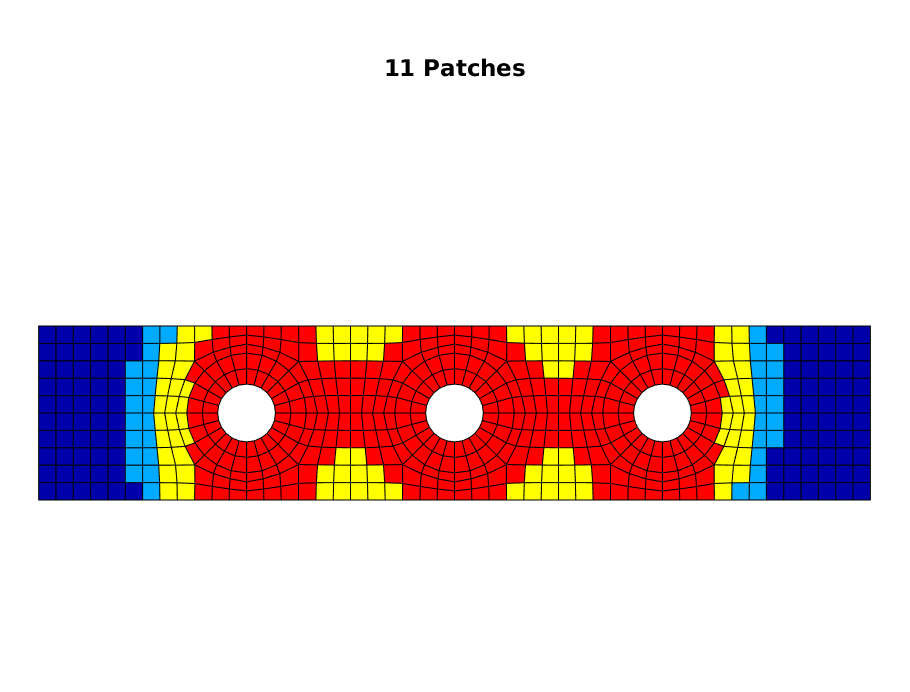
\includegraphics[width=0.9\linewidth,trim={1cm 2.95cm 1cm
    %     5.2cm},clip]{{{FIGS/P11580_S-6.00_4LEV_11PATCH_MESH}}}}
    \boxed{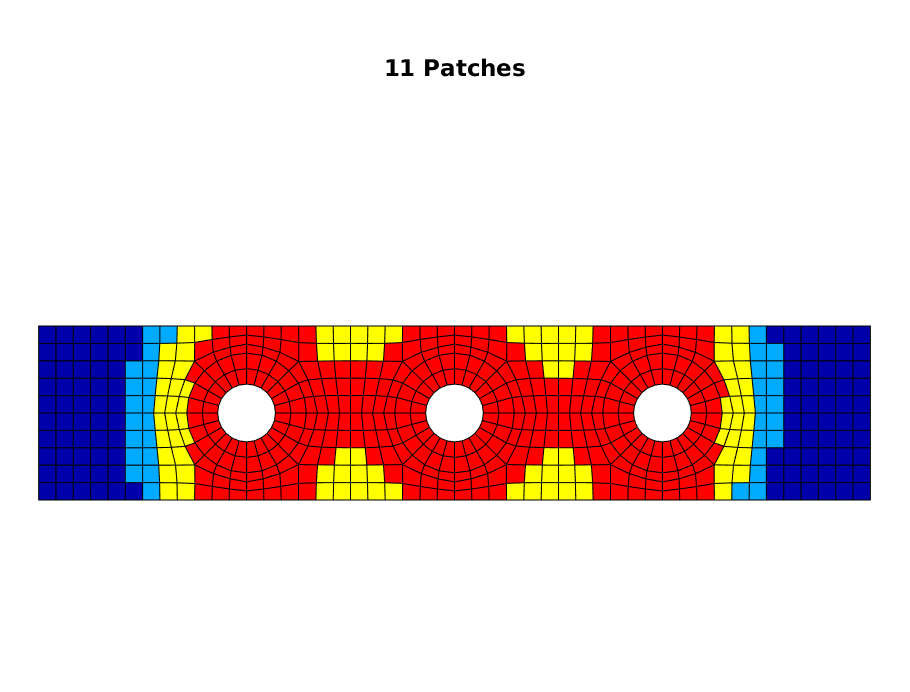
\includegraphics[width=0.9\linewidth,trim={1cm 2.95cm 1cm
        5.2cm},clip]{8621_bal_Fig2b}}
    \caption{4 Levels (11 Patches)}
  \end{subfigure}%

  \begin{subfigure}{0.5\linewidth}
    \centering
    % \boxed{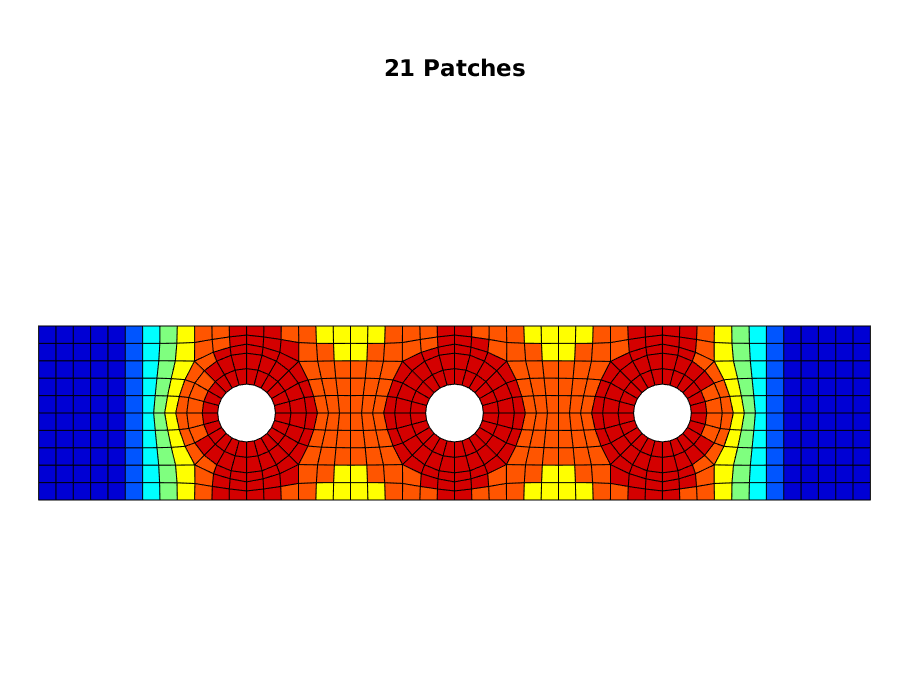
\includegraphics[width=0.9\linewidth,trim={1cm 2.95cm 1cm
    %     5.2cm},clip]{{{FIGS/P11580_S-6.00_7LEV_21PATCH_MESH}}}}
    \boxed{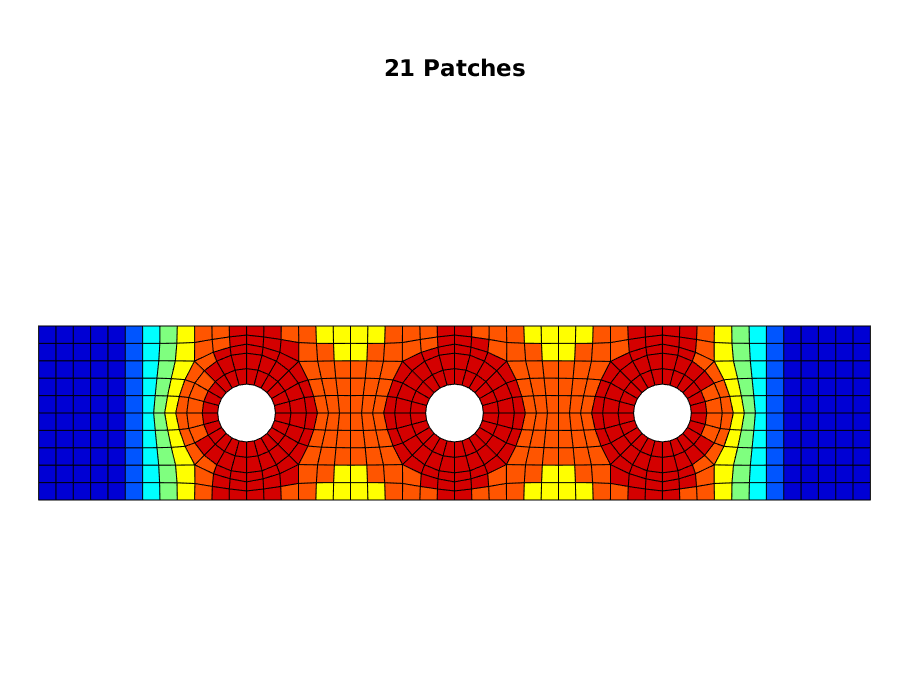
\includegraphics[width=0.9\linewidth,trim={1cm 2.95cm 1cm
        5.2cm},clip]{8621_bal_Fig2c}}
    \caption{7 Levels (21 Patches)}
  \end{subfigure}%  
  \caption{Binned objective patches for the Brake-Reu{\ss} Beam
    (BRB) interface. The colors indicate different patches.}
  \label{fig:wja}
\end{figure}

For the first approach, the field $\mathcal{P}(\utilde{x})$ is first
divided into a set of discrete levels $\mathcal{P}_{min} =
\mathcal{P}_0<\mathcal{P}_1<\dots<\mathcal{P}_{N_{lev}}=\mathcal{P}_{max}$. Elements
corresponding to each bin $i$ are selected as the elements that have
$\mathcal{P}(\utilde{x})\in[\mathcal{P}_{i-1},
\mathcal{P}_i)$. Following this, disconnected trees of the ensuing
graph are identified and separated into separate
``patches''. Repeating this procedure for all the chosen levels yields
a set of patches (defined as element-sets).

An improved stiffness-preserving whole-joint
formulation\footnote{Similar, but not identical to the RBE3 elements
  in ANSYS terminology} (see~\cite{intredpaper} for formulation) is
then employed to represent each of these patches by a single
six-Degree-of-Freedom (six-DoF) virtual node (three displacements and
three rotations). Finally, conducting a CMS (Component-Mode Synthesis)
procedure on this gives the effective reduced order model. Since this
is a model that is based on a set of physical DoF's, contact models
may be used on these nodes directly (making the model
hyper-reduced).

\Cref{fig:wja} indicates the patches identified for three different
binning levels for the interface of .

\subsection{Interface Remeshing Approach}
\label{sec:interf-remesh-appr}

The second approach comes from the idea that not all nodes in an
interface may be necessary to accurately represent a field
variable. Therefore, information about the local gradients of the
field quantity are employed to guide the design of a new mesh on top
of the initial mesh in the interface. Consider a ``full mesh'',
  denoted by $\mathcal{T}$, and a ``reduced mesh'', denoted by
  $\mathcal{T}_r$. Denoting the nodal DoF vectors in each as
  $\utilde{u}$ and $\utilde{u_r}$ respectively, the vector
  $\utilde{u}$ may be approximated by interpolating $\utilde{u_r}$ on
  the mesh $\mathcal{T}_r$ using its shape functions as follows:
\begin{equation}
  \utilde{u} \approxeq \mathbf{Q}_r\utilde{u_r}.
  \label{eq:interp}
\end{equation}
Here, the matrix $\mathbf{Q}_r$ denotes the interpolation matrix
developed using the corresponding shape functions of
$\mathcal{T}_r$. Note that the same relationship (in~\cref{eq:interp})
may be used to approximate nodal tractions on the original mesh but
not forces.

For a dynamical system of the form
  \begin{equation}
    \label{eq:dynsys}
    \mathbf{M} \ddot{\utilde{u}} + \mathbf{K} \utilde{u} +
    \utilde{f_{nl}}(\utilde{u}) = \utilde{f_{ext}}(t),
  \end{equation}
  a Galerkin-projection-based Reduced-Order-Model (ROM) may be
  developed if~\cref{eq:interp} is interpreted as a projection onto a
  reduced basis. \Cref{eq:dynsys}, under this projection, becomes
  \begin{equation}
    \label{eq:ROMsys}
    \left[{\mathbf{Q}_r}^T \mathbf{M} \mathbf{Q}_r\right]
    \ddot{\utilde{u_r}} + \left[{\mathbf{Q}_r}^T \mathbf{K}
      \mathbf{Q}_r\right] \utilde{u_r} + \underbrace{{\mathbf{Q}_r}^T 
    \utilde{f_{nl}}(\mathbf{Q}_r\utilde{u_r})}_{\utilde{f_{nl}^{r}}} =
  {\mathbf{Q}_r}^T \utilde{f_{ext}}(t).
  \end{equation}
  Note here that the non-linear force $f_{nl}$ still has to be
  evaluated as many times as in the original model, i.e., the model is
  not hyper-reduced yet. This is achieved by evaluating the non-linear
  tractions in $\mathcal{T}_r$ (denoted as $t_r(\utilde{u_r})$),
  interpolating it onto $\mathcal{T}$ (becoming
  $\mathbf{Q}_rt_r(\utilde{u_r})$), integrating this in on
  $\mathcal{T}$ (computed with some quadrature integration matrix
  $\mathbf{P}$ and denoted as
  $\mathbf{P}\mathbf{Q}_rt_r(\utilde{u_r})$), and finally applying the
  Galerkin projection to obtain the forcing for the ROM. This
  procedure may be summarized as,
  \begin{equation}
    \label{eq:hyperred}
    \utilde{f_{nl}^r} = {\mathbf{Q}_r}^T
    \utilde{f_{nl}}(\mathbf{Q}_r\utilde{u_r}) =
    \underbrace{{\mathbf{Q}_r}^T\mathbf{P}\mathbf{Q}_r}_{\mathbf{T}_m^f}t_r(\utilde{u_r}).
  \end{equation}
  Here, the non-linearities need to be evaluated only in the reduced
  mesh $\mathcal{T}_r$, and projected onto the ROM using a single
  matrix $\mathbf{T}_m^r$. Since integrals of tractions on
  $\mathcal{T}_r$ directly do not have any meaning for the ROM, the
  reduced mesh may not be interpreted as a regular finite element mesh
  that discretizes the interface in a reduced fashion. It merely
  represents a reduced representation of the original mesh with
  consistent (but approximate) mappings.

\begin{figure}[!h]
  \centering
  \begin{subfigure}{0.5\linewidth}
    \centering
    % \boxed{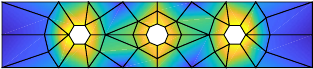
\includegraphics[width=0.9\linewidth]{FIGS/P52}}
    \boxed{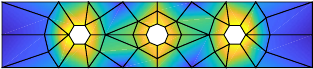
\includegraphics[width=0.9\linewidth]{8621_bal_Fig3a}}
    \caption{52 Elements}
  \end{subfigure}%  
  \begin{subfigure}{0.5\linewidth}
    \centering
    % \boxed{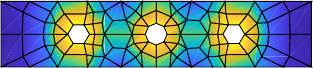
\includegraphics[width=0.9\linewidth]{FIGS/P124}}
    \boxed{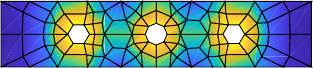
\includegraphics[width=0.9\linewidth]{8621_bal_Fig3b}}
    \caption{124 Elements}
  \end{subfigure}
  
  \begin{subfigure}{0.5\linewidth}
    \centering
    % \boxed{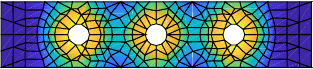
\includegraphics[width=0.9\linewidth]{FIGS/P300}}
    \boxed{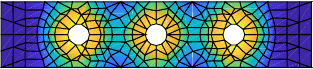
\includegraphics[width=0.9\linewidth]{8621_bal_Fig3c}}
    \caption{300 Elements}
  \end{subfigure}
  \caption{Examples of different reduced meshes using approach 2. The
    colors indicate the field-objective function, with blue indicating
    0 and yellow indicating 1.}
  \label{fig:ira}
\end{figure}
\vspace{-0.2cm}
\Cref{fig:ira} presents sample reduced meshes developed for the BRB
interface using the contact pressure as the objective field 
(see~\cref{fig:iraref} for the field on full mesh). The pressure
values are re-scaled to range from 0 to 1 for convenience. For the
meshes shown in the figure, nodes were biased to lie in regions with
large gradients or changes in the objective field.

\section{Results}
\label{sec:results}

\begin{figure}[!h]
  \centering
  \begin{subfigure}{0.5\linewidth}
    % 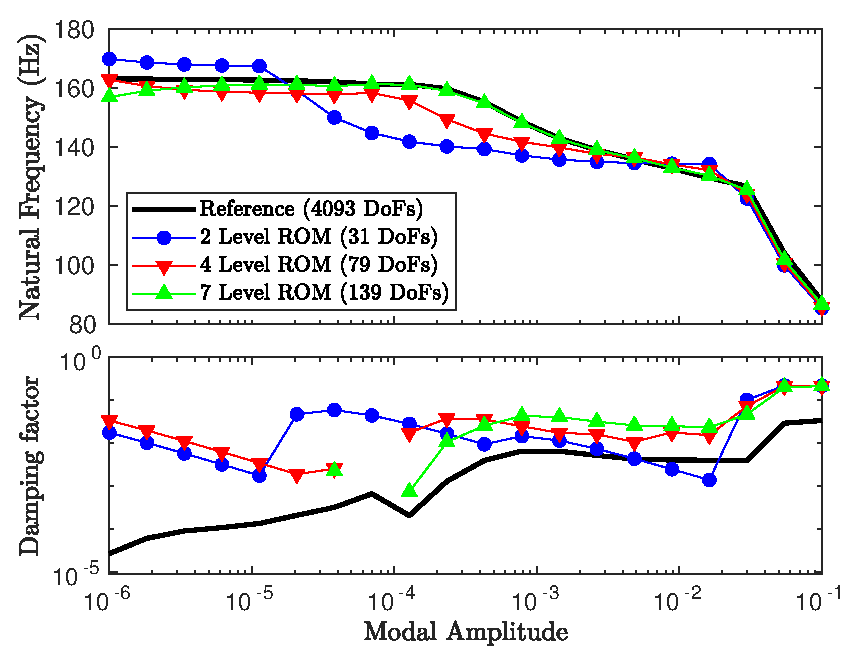
\includegraphics[width=\linewidth]{{{FIGS/P11580_S-6.00_ELDRYFRICT_BB_WJROM}}}
    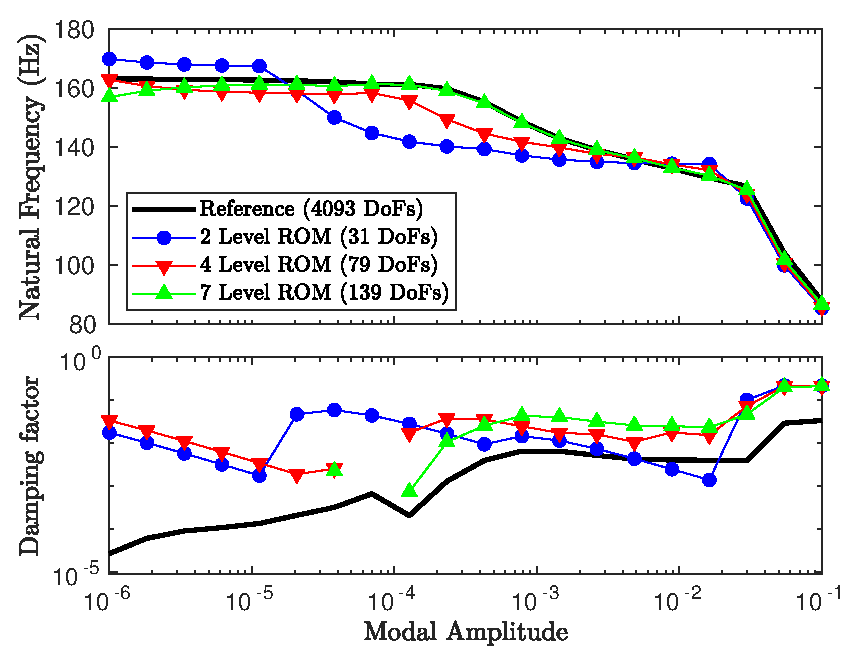
\includegraphics[width=\linewidth]{8621_bal_Fig4a}
    \caption{}
  \end{subfigure}%
  \begin{subfigure}{0.5\linewidth}
    % 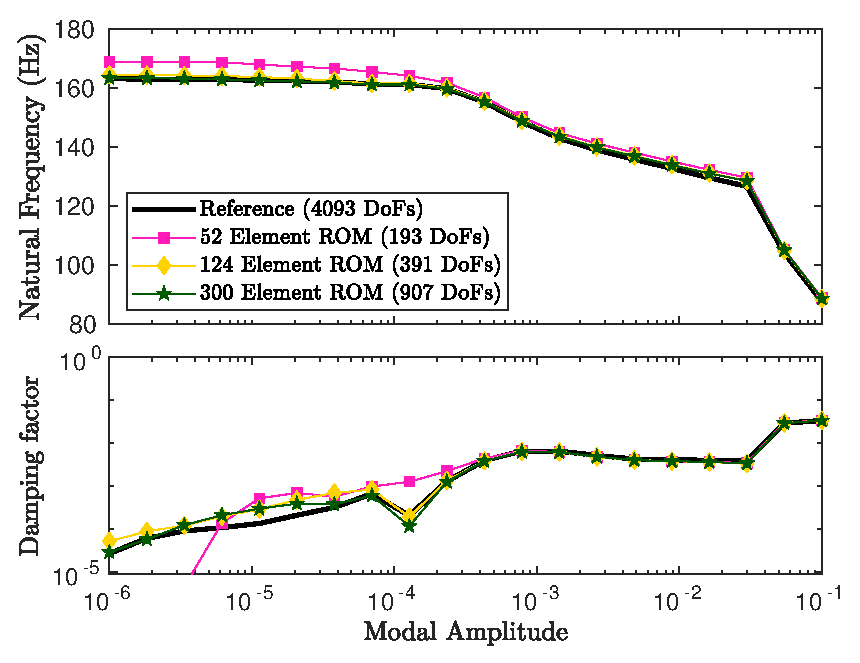
\includegraphics[width=\linewidth]{{{FIGS/P11580_S-6.00_ELDRYFRICT_BB_FJROM}}}
    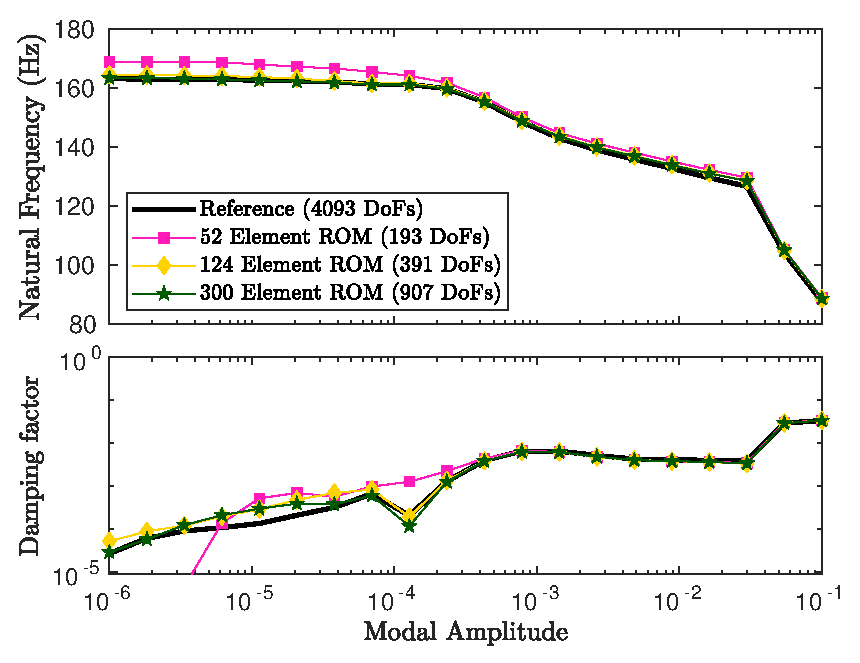
\includegraphics[width=\linewidth]{8621_bal_Fig4b}
    \caption{}
  \end{subfigure}
  \caption{Results for the (a) Whole Jointed Approach and the (b)
    Remeshing approach. Reference results are calculated using the
    full mesh (\cref{fig:iraref}); whole joint ROMs are developed
    based on the patches shown in~\cref{fig:wja}; and remeshing ROMs
    are developed based on the meshes shown in~\cref{fig:ira}.}
  \label{fig:res}
\end{figure}

\Cref{fig:res} shows the results for amplitude-dependent non-linear
modal simulations using the technique developed in~\cite{rqnm} for the
first mode of vibration. Unilateral linear springs and planar elastic dry
friction elements (2D Jenkins models) are used in the traction-sense
as the normal and tangential contact constitutive relationships for
the reference model and the remeshing ROMs. The same contact laws are
employed for the whole joint ROMs but since these require
phenomenological models (force-displacement models), the
traction-stiffnesses used in the reference are scaled by the areas of
each patch to obtain consistent model parameters for the ROMs.

In terms of performance, one can see that both demonstrate good
convergence in capturing the reference trends in the stiffness
characteristics (amplitude-dependent natural frequency). However, the
remeshing approach seems to represent the dissipative characteristics
(amplitude-dependent damping factor) much better than the whole joint
approach. This may be an observation that could be related to the
formulations of the ROMs, or just numerical relics of the estimated
dissipation metric. Further investigations are currently being
conducted to draw more conclusions.

\section{Discussions and Conclusions}
\label{sec:disc-concl}

The paper presents the development and relative comparison of
hyper-reduction approaches for structures with small displacement
contacting interfaces. The ROMs developed are consistently
hyper-reduced, i.e., simulations of the full non-linear model are not
necessary for the hyper-reduction. An additional advantage of this is
that a developed ROM can potentially be used to conduct cheap
simulations over any amplitude range of interest accurately.

In addition to extracting conclusive inferences from observations such
as in~\cref{sec:results}, the current investigation also explores the
use of different choices of objective functions such as modal strains
from linear modal analyses, dissipation fields from non-linear modal
analyses, etc., as well as weighted combinations of these.

Another aspect that is taken up in the current work is the fact that
it may not always be possible to come up with asymptotic accuracy
analyses for the approaches considered here. For the first approach,
having a very large number of binning levels leads to a system
where some patches will be constituted with just a single
element. These present numerical difficulties since in this case all
the nodes will be shared by the patch with adjacent patches. For the
second approach, increasing the number of required elements starts
failing after a point since the elements one can come up with, while
following the specified objective, start losing
shape-regularity and yield bad quality elements. In most cases,
  however, this has been encountered when the sizes of some elements
  in the reduced mesh start becoming significantly smaller than those
  of the reference mesh.

\bibliographystyle{plainnat}
\bibliography{8621_bal_refs}
\end{document}
%%% Local Variables:
%%% mode: latex
%%% TeX-master: t
%%% End:
